\section{Teoretická časť}

\subsection{Odporúčacie systémy}
\label{sec:odporucacie systemy}
 Odporúčacie systémy predstavujú softvérové nástroje a techniky, ktoré poskytujú používateľovi odporúčania ohľadom daného súboru položiek. Odporúčania súvisia s rôznymi rozhodovacími procesmi, ako napríklad akú položku kúpiť, akú hudbu počúvať alebo aké online noviny čítať. Dalo by sa teda povedať, že ich hlavným cieľom je odporučiť danému používateľovi jemu relevantné položky. "Položka" je termín, ktorý označuje čo konkrétne daný odporúčací systém odporúča používateľom. Vzhľadom nato, že odporúčania sú väčšinou personalizované, rôzny používatelia dostávajú rozličné odporúčania. Existujú aj nepersonalizované odporúčania. Tie fungujú na jednoduchšom princípe a je ľahšie ich generovať. Typickým príkladom sú rebríčky, ktoré obsahujú výber top 10 najobľúbenejších položiek. \cite{rs1} 
 
Väčšina veľkých internetových služieb ako Amazon, YouTube, Netflix, Google, Tripadvisor či \acrshort{imdb}, majú vyvinuté svoje vlastné odporúčacie systémy, ktoré dlhodobo pomáhajú zlepšovať ich výsledky, ale aj \acrshort{ux}. Netflix v roku 2009 odmenil tím programátorov, ktorý ako prvý úspešne zefektívnil ich odporúčací systém o takmer 10\%, cenou 1 milión dolárov. To len zvýrazňuje ich významnosť a fakt, že svetové firmy do tejto technológie investujú nemalé finančné prostriedky. \cite{rs1}

Existuje viacero dôvodov, prečo poskytovatelia služieb využívajú túto technológiu: 
 \begin{itemize}[leftmargin=*]
{\bf \item Zvýšenie predaja} - najdôležitejšia funkcia pre komerčný odporúčací systém, je prirodzene zvýšenie počtu predaných položiek. Čím efektívnejší je, tým lepšie výsledky firme generuje. 

{\bf \item Predávať rôznorodý tovar} - ďalšia významná funkcia je umožniť používateľovi vybrať si položky, ktoré by bez odporúčania našiel ťažšie. 
 
{\bf \item Zvýšiť spokojnosť používateľa} - dobre fungujúci odporúčací systém, vie zlepšiť aj celkový \acrshort{ux}, čo v konečnom dôsledku zabezpečí, že používateľ bude služby rád využívať. 

{\bf \item Zvýšiť vernosť používateľa} - akonáhle používateľ zaregistruje, na základe presných odporúčaní, že ho služba "pozná", nadobudne pocit, že ho považuje za hodnotného zákazníka a bude sa rád vracať.
	
{\bf \item Lepšie rozumieť tomu, čo zákazník chce} - pomocou zbierania rôznych používateľských preferencií a následného analyzovania, vedia firmy lepšie reagovať na trh a zmeny na ňom a tým prispôsobovať svoj sortiment potrebám trhu. \cite{rs1} \newline

\end{itemize} 


\subsubsection{Základné pojmy}
Všeobecná klasifikácia dát použitých v odporúčacích systémoch rozlišuje 3 druhy objektov.
 \begin{itemize}[leftmargin=*]
{\bf \item Položky} - sú objekty ktoré sú odporúčané. Môžu byť charakterizované ich zložitosťou a ich hodnotou alebo užitočnosťou. Hodnota môže byť kladná, ak je položka pre používateľa užitočná, alebo záporná, ak položka nie je vhodná. 
{\bf \item Používatelia} - môžu mať veľmi rozdielne ciele a vlastnosti. S cieľom personalizovať odporúčania a interakciu, odporúčacie systémy využívajú množstvo informácií o používateľoch.
{\bf \item Transakcie} - všeobecne označujeme ako zaznamenanú interakciu medzi používateľom a odporúčacím systémom. Sú to dáta podobného typu ako logy, ktoré uchovávajú dôležité informácie vygenerované počas interakcie, ktoré sú užitočne pre odporúčací algoritmus. \cite{rs1}
\end{itemize} 


Vo všeobecnosti, existujú odporúčacie techniky, ktoré nevyžadujú veľké množstvo vedomostí tj. používajú veľmi jednouché základné dáta, ako napríklad používateľove hodnotenia. Tieto hodnotenia môžu byť zbierané explicitne, alebo implicitne. Implicitne je možno získať údaje napríklad z histórie nákupov, alebo použiť ako indikátor množstvo času, ktoré používateľ strávi prehliadaním konkrétneho typu položky. Hodnotenia môžu byť v rôznych formách, ako napríklad: \cite{rs1}
 \begin{itemize}[leftmargin=*]
{\item numerické hodnotenie na pevne stanovenej stupnici (napr. 1-5),} 
{\item slovné hodnotenia ako veľmi súhlasím, súhlasím, neutrálny, nesúhlasím, veľmi nesúhlasím,} 
{\item jednoduché binárne hodnotenie (dobré/zlé)} \cite{rs1}
\end{itemize} 

Niektoré odporúčacie systémy nemusia nutne odhadovať užitočnosť položiek priamo pred ich odporúčaním, ale môžu namiesto toho použiť určitú formu heuristiky, aby vytvorili hypotézu, že položka je pre používateľa užitočná. Tieto predikcie užitočnosti sú vypočítané špecifickými algoritmami a využívajú rozličné druhy vedomostí, ktoré systém má o používateľoch a položkách. \cite{rs1} \\

\subsubsection{Typy odporúčacích systémov}
\begin{itemize}[leftmargin=*]
{\bf \item Demografické - }Tento typ systémov odporúča položky na základe demografického
profilu používateľa, teda oblasti v ktorej sa nachádza. 
{\bf \item Knowledge-based - }Systémy založené na znalostiach, odporúčajú položky na základe konkrétnych znalostí o tom, ako určité vlastnosti položiek zodpovedajú potrebám a preferenciám používateľov.
{\bf \item Komunitné - }Odporúčanie je založené na preferenciách užšej komunity okolo používateľa, častokrát označovanej ako priatelia. Tento typ systému dobre vystihuje epigram „Povedzte mi, kto sú vaši priatelia a ja vám poviem, kto ste.“ Prieskumy naznačujú, že ľudia sa skôr spoliehajú na odporúčania svojich priateľov než na anonymné odporúčania. \cite{communityrec} Toto pozorovanie v kombinácii s popularitou sociálnych sietí vytvára rastúci záujem o komunitné systémy označované aj ako sociálne odporúčacie systémy. \cite{rs1}\\
\end{itemize} 
 
\subsubsection{Typy odporúčacích techník}
Pri odporúčacích systémoch existujú dve hlavné techniky návrhu algoritmu a to kolaboratívne filtrovanie a filtrovanie na základe obsahu.\\

\subsubsection{Kolaboratívne filtrovanie (collaborative filtering)}
Kolaboratívne filtrovanie je technika, ktorá vytvára odporúčania na základe zbierania preferencií od väčšieho počtu používateľov. Odporúča používateľovi položky, ktoré v minulosti pozitívne ohodnotili používatelia s podobnými preferenciami \hyperref[collaborativeFiltering]{(pozri obr. \ref{collaborativeFiltering})}. 

Teda ak máme používateľa  \textit{u}, tak jeho hodnotenie položky \textit{i} je pravdepodobne podobné, ako hodnotenie tej istej položky \textit{i} iným používateľom \textit{v}, pokiaľ \textit{u} a \textit{v} hodnotili iné položky podobne. Treba poznamenať, že tieto predpovede sú špecifické pre daného používateľa, ale vytvárajú sa na základe informácií zhromaždených od veľkého počtu iných používateľov. Kolaboratívne filtrovanie je považované za najpopulárnejšiu techniku používanú v odporúčacích systémoch. \cite{rs1} \\\\\\


\begin{figure}[!htbp]
  \centering  
  \def\stackalignment{c}
	\stackunder{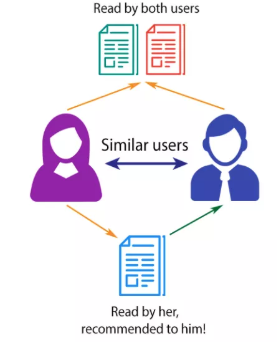
\includegraphics[width=7cm]{img/colaborative filtering.png}}%
           {\scriptsize%
            Zdroj: \cite{rs3}}
  \caption{Kolaboratívne filtrovanie}
  
  \label{collaborativeFiltering}
\end{figure}

Existujú dva prístupy pri používaní tejto techniky:
\begin{enumerate}
	{\bf \item Pamäťové metódy (memory-based methods)} sú metódy v ktorých hodnotenia položiek používateľom, sú predpovedané na základe jeho susedov. Týchto susedov môžeme ďalej definovať dvoma spôsobmi: \cite{rs3}
\begin{itemize}[leftmargin=*]
	{\bf \item Zamerané na používateľov (user-based)}\newline	
Predpovedá hodnotenie položky \textit{i} používateľom \textit{u}, použitím hodnotení \textit{i} od iných používateľov, ktorí sú čo najviac podobní \textit{u}. \cite{rs1} Inak povedané snaží sa nájsť iných podobných používateľov (susedov) a odporúčať používateľovi \textit{u} produkty ktoré sa páčia im.
	{\bf \item Zamerané na položky (item-based} \newline
Zatiaľ čo pri user-based metóde sa pri predpovedaní hodnotenia spoliehajú na názor rovnako zmýšľajúcich používateľov, item-based prístupy sa zameriavajú na hodnotenie udelené podobným položkám. Túto myšlienku môžeme sformalizovať nasledovne. Predpoveď hodnotenia položky \textit{i} používateľom \textit{u}, môžeme získať ako vážený priemer hodnotení, ktoré \textit{u} dal iným položkám, ktoré sú čo najviac podobné \textit{i}. \cite{rs1}
\end{itemize}
	{\bf \item Model-based methods} využívajú metódy strojového učenia na tvorbu predpovedí. Využívajú sa techniky ako \acrshort{pca}, \acrshort{svd}, faktorizácia matíc, clusterin či neurónové siete. \cite{rs3} \\
\end{enumerate}

Kolaboratívne filtrovanie, prináša jeho používaním zaujímavé výhody. Spomenieme tie najpodstatnejšie z nich. Veľkou výhodou je, intuitívnosť a relatívne jednoduchá implementácia. V jeho najjednoduchšej podobe vyžaduje vyladenie iba jeden parameter (počet susedov použitých v predikcii). Dôležitá je aj stabilita, keďže takéto systémy sú veľmi málo ovplyvnené neustálym pridávaním nových používateľov, položiek a hodnotení, čo sa zvyčajne vyskytuje vo veľkých komerčných aplikáciách.
Zaujímavou možnosťou je aj zlepšenie \acrshort{ux} tým, že používateľovi ako odôvodnenie odporúčaní zobrazíme zoznam susedových položiek, ako aj hodnotenie, ktoré týmto položkám dal. To môže pomôcť používateľovi lepšie pochopiť odporúčanie resp. jeho relevantnosť a môže slúžiť ako základ pre interaktívny systém, kde si môžu používatelia vybrať susedov, ktorým by sa mala venovať väčšia dôležitosť. \cite{rs1} \\


Hlavnou nevýhodou týchto systémov je tzv. "cold start problem", čo znamená, že je takmer nemožné niečo odporučiť novému používateľovi, alebo odporúčať novú položku používateľom. Navyše mnoho používateľov a položiek má príliš málo interakcií nato, aby algoritmus s nimi vedel efektívne pracovať. Riešenia tohto problému bývajú, že novým používateľom sa odporúčajú náhodné položky a nové položky sa odporúčajú náhodným používateľom (tzv. "random strategy"). Často sa používa aj odporúčanie populárnych položiek novým používateľom a odporúčanie nových položiek najviac aktívnym používateľom (tzv. "maximum expectation strategy"). V skorej fáze "života" používateľa alebo položky, sa môže použiť iná metóda ako kolaboratívne filtrovanie. \cite{rs2} \\
	
 
\subsubsection{Filtrovanie na základe obsahu (content based filtering)}
\label{sec:contentbased}
Táto technika zahŕňa odporúčanie položiek na základe ich samotných vlastností. \cite{rs3} Odporúčania sú tu vytvárané na základe predchádzajúcich interakcií jednotlivých používateľov s položkami. Systém pracujúci touto metódou, sa snaží hľadať podobnosti medzi položkami, s ktorými mal používateľ v minulosti pozitívnu interakciu (t.j. kúpil si daný produkt, ohodnotil kladne daný film, pridal skladbu do obľúbených atď.). Napríklad ak používateľ pozitívne ohodnotí film zo žánru komédia, systém z toho môže vyčítať, že do jeho preferencií patrí aj tento žáner a teda mu odporúčať komediálne filmy. \cite{rs1} Princíp fungovania je znázornený na \hyperref[contentFiltering]{obrázku \ref{contentFiltering}}.

Nato aby táto technika správne fungovala, si systém musí vytvoriť pri danom používateľovi akýsi model, resp. profil, ktorý reprezentuje používateľove preferencie, ktoré získa na základe vlastností pozitívne hodnotených položiek. Napríklad pri odporúčaní filmov, vlastnosti, ktoré opisujú film sú herci, režiséri, žánre, hodnotenie filmu atď. Tieto vlastnosti sa zvyknú označovať aj ako atribúty. Proces tvorby odporúčaní potom pozostáva z hľadania zhody medzi atribútmi profilu a atribútmi prehľadávaných položiek. \cite{rs1} \\\\
\begin{figure}[!htbp]
  \centering  
  \def\stackalignment{c}
	\stackunder{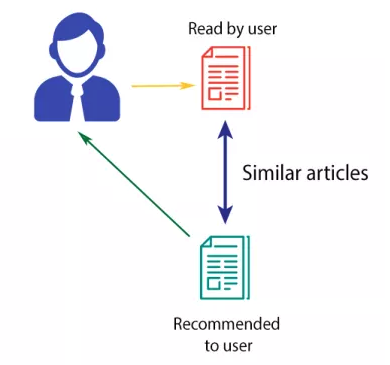
\includegraphics[width=7cm]{img/content-based-filtering.png}}%
           {\scriptsize%
            Zdroj: \cite{rs3}}
  \caption{Filtrovanie na základe obsahu}
  
  \label{contentFiltering}
\end{figure}

Spomeňme hlavné výhody, ktoré prináša použitie tejto metódy. Nezávislosť od používateľov je dosiahnutá vďaka tomu, že profil používateľa, na základe ktorého sa hľadajú zhody s položkami, je vytvorený len z hodnotení položiek daným používateľom. Zistiť ako systém funguje, je možné pomocou atribútov, ktoré model zohľadňuje pri vytváraní profilu. To vie pomôcť pri porozumení, prečo sa konkrétna položka objavila v zozname odporúčaných. V tejto metóde je možné odporúčať aj novú položku, ktorá nebola ešte hodnotená žiadnym používateľom. Vďaka tomu netrpí "cold-start" problémom, ktorý postihuje kolaboratívny filtering. \cite{rs1} \\

Napriek spomenutým výhodám, použitie tejto techniky prináša aj isté obmedzenia. Nato aby systém dokázal naozaj dobre porozumieť používateľovým preferenciám a vytváral presné odporúčania, je nevyhnutné mať zozbieraných dostatok hodnotení. Pri nových používateľoch, ktorí majú zo začiatku málo hodnotení, systém väčšinou neprináša spoľahlivé odporúčania. 

Nežiadúcou vlastnosťou je tiež aj tzv. "serendipity problem", čím sa zdôrazňuje tendencia systému produkovať odporúčania, ktoré sa často podobajú a neobmieňajú. Napríklad ak používateľ pozitívne hodnotil filmy od režiséra Stanleyho Kubricka, v odporúčaniach mu môžu prevažovať filmy tohto režiséra. \cite{rs1} \\

\subsubsection{Zdôvodnenie výberu}
Ako základ nášho systému sme si vybrali filtering na základe obsahu. Pri filmoch sa dá vybrať mnoho atribútov, pomocou ktorých si vieme jednoducho vytvoriť profil preferencií daného používateľa. Kolaboratívny filtering aj vzhľadom na malý počet používateľov neprichádzal do úvahy.

\subsection{Mobilné aplikácie}
Mobilná aplikácia je softvérová aplikácia vytvorená špecificky pre mobilné zariadenia ako napríklad smartfóny, tablety alebo inteligentné hodinky. \cite{ma1} Pôvodne boli aplikácie vytvárané výrobcami mobilných operačných systémov, ktorí potrebovali pre používateľov zjednodušiť používanie základných funkcií smartfónu, ako napríklad prezeranie emailov, správ o počasí, prácu s kalendárom, fotenie fotografií atď. \cite{ma2} Avšak, vďaka rýchlemu vývinu samotných smartfónov a ich operačných systémov, začal rásť dopyt aj po aplikáciách zameraných na iné oblasti. V dnešnej dobe sú najpopulárnejšie rôzne herné aplikácie, navigačné aplikácie, aplikácie na online komunikáciu, hudobné aplikácie a mnohé iné. V posledných rokoch si používanie smartfónu bez spomenutých aplikácií ani nevieme predstaviť a stali sa ich neoddeliteľnou súčasťou. Aplikácie sa väčšinou sťahujú z distribučných platforiem, ktoré sú prevádzkované vlastníkom daného operačného systému, na ktorý je aplikácia určená. Spomeniem dva najväčšie a to App Store patriaci pod operačný systém iOS a Google Play Store patriaci pod Android. Na oboch platformách vieme nájsť veľké množstvo aplikácií všemožného zamerania, pričom každým dňom pribúdajú ďalšie. \cite{ma1} \\
\subsubsection{Typy mobilných aplikácií}
\label{sec:typy aplikacii}
Vo všeobecnosti sa mobilné aplikácie delia na 4 základné kategórie. Natívne, webové, hybridné a cross platformové aplikácie.
\begin{itemize}[leftmargin=*]
{\bf \item Natívne aplikácie} - sú vytvorené výlučne pre špecifický mobilný operačný systém tj. natívne Android aplikácie alebo natívne iOS aplikácie. Kvôli špecifickému zameraniu na jeden operačný systém nie je možné aplikácie kombinovať na rôznych platformách. Napríklad Blackberry aplikácia nie je spustiteľná na Androide, Android aplikáciu zase nespustíme na iOS. Teda všeobecne povedané, mobilnú aplikáciu nainštalujete a spustíte len na operačnom systéme, pre ktorý je vytvorená. Inštalujú sa priamo do mobilného zariadenia, potrebné dáta sú väčšinou uložené priamo v internom úložisku zariadenia. \cite{ma3} \\

{\bf Používané technológie:} Na vývoj natívnych aplikácií sa používajú viaceré programovacie jazyky podľa toho, pre aký \acrshort{os} majú byť určené. Medzi najpoužívanejšie patria Java a Kotlin pre Android, Swift a Objective-C pre iOS. \\

{\bf Výhody:} Vďaka tomu, že sú zamerané na jednu platformu, vedia byť z hľadiska výkonu rýchlejšie a stabilnejšie. Hardvér zariadenia vedia využívať efektívnejšie. Sú schopné priamo pristupovať k všetkým funkciám zariadenia, vďaka čomu vedia využiť širokú ponuku možností, ktoré dané zariadenie ponúka ako napríklad fotoaparát, kontakty zariadenia, bluetooth, \acrshort{nfc} či dokonca samotnú polohu zariadenia (\acrshort{gps}). Veľkú obľubu im zabezpečuje aj to, že využívajú natívny \acrshort{ui}, čo prináša používateľom lepší \acrshort{ux}. \cite{ma3} \\
 
{\bf Nevýhody:} Primárnym problémom je duplicita pri vývoji aplikácie, keďže je potrebné aplikáciu naprogramovať pre viaceré mobilné operačné systémy, čo priamoúmerne zvyšuje cenu nehovoriac o náročnosti údržby a aktualizácie kódu pri každej novej verzii. Menší komfort spôsobuje aj fakt, že ak používateľ nechce prísť o najnovšiu funkcionalitu a opravu chýb, mal by pri každej aktualizácií aplikáciu preinštalovať resp. si nainštalovať tzv. update. \cite{ma3} \\

{\bf \item Webové aplikácie} - sú to v podstate responzívne webové stránky, ktoré sa prispôsobujú svojim vzhľadom zariadeniu na ktorom sú spustené. \cite{ma3} \\

{\bf Používané technológie:} Webové aplikácie sú vytvorené pomocou jazyka \acrshort{html}, jej vzhľad je naštýlovaný pomocou \acrshort{css} a dynamické správanie zabezpečuje JavaScript. \\

{\bf Výhody:} Keďže na svoje fungovanie využívajú webový prehliadač, zaniká problém duplicity pri programovaní aplikácie na viaceré operačné systémy. Toto znižuje náročnosť či už na vývoj, alebo cenu. \cite{ma3} \

{\bf Nevýhody:} Hlavná nevýhoda pramení už z názvu - webové aplikácie, z čoho vyplýva, že bez internetového pripojenia ich nieje možné využívať. Webový prehliadač vie tiež ovplyvniť \acrshort{ux}. Kým v jednom zariadení môže byť k dispozícií plná funkcionalita, môže sa stať, že na druhom už len obmedzená. Programátori sa tomu samozrejme snažia zabrániť a programovať aplikácie tak, aby boli plne funkčné na čo najväčšom množstve najviac používaných prehliadačov a zariadení. Nevýhodou je tiež značne obmedzený prístup k pokročilejším funkciám zariadenia ako napríklad využívanie gest, polohy zariadenia či \acrshort{nfc}. \cite{ma3} \\
 
{\bf \item Hybridné aplikácie} - sú založené na princípe miešania prvkov natívnych a webových aplikácií. Jadro aplikácie je napísane pomocou webových technológií (\acrshort{html}, \acrshort{css}, JavaScript), pričom je spúšťané z natívnej aplikácie a jej vlastného zabudovaného prehliadača, ktorý je ale pre používateľa neviditeľný. Napríklad aplikácia pre iOS by na zobrazenie používala WKWebView objekt, zatiaľ čo v Androide by na vykonávanie rovnakej funkcie používala WebView objekt. Kód samotný, je potom vložený do kontajnera natívnej aplikácie s použitím frameworkov ako Apache Cordova (známy aj ako PhoneGap), alebo Ionic. Tieto frameworky navyše majú aj systém pluginov, ktorý umožňuje ľahko prekonať obmedzenia webových aplikácií a rozšíriť funkcionalitu nad rámec prehliadača. Aplikácia tak môže získať plnú kontrolu nad funkciami mobilného zariadenia, čo umožňuje napríklad použiť TouchID pri iOS ako možnosť prihlásenia sa do aplikácie. \cite{ma4} \\


{\bf Používané technológie:} Hybridné aplikácie používajú kombináciu webových technológií a natívnych \acrshort{api}. Sú vyvinuté pomocou technológií ako Ionic, Apache Cordova, Swift, \acrshort{html}5, \acrshort{css}, a JavaScript. \cite{ma3} \\

{\bf Výhody:} Kombinácia dobrého \acrshort{ux}, menšej náročnosti pri vývoji a prijateľná cena, sú často hlavné činitele v ktorých hybridné aplikácie predčia konkurenciu. Vďaka tomu, že je z veľkej časti použitý rovnaký zdrojový kód, nezávisle od mobilného operačného systému. Na vývoj je potrebných menej vývojárov (napr. nemusia byť zvlášť tímy vývojárov pre iOS a zvlášť pre Android). \cite{ma4} \\
 
{\bf Nevýhody:} Najväčším mínusom hybridných aplikácií je výkon. Keďže sa načítavajú v spomínanom WebView objekte podobnom webovému prehliadaču, sú vysoko závislé od jeho samotného výkonu keďže je zodpovedný za zobrazovanie \acrshort{ui} a beh kódu. Napriek tomu, že aplikácie vedia bežať na viacerých operačných systémoch, je vcelku náročné si túto vlastnosť udržať. Občas vďaka výdavkom na implementáciu cross platformingu, vie cena hybridnej aplikácie dosiahnuť ceny natívnych aplikácií. \cite{ma4} \cite{ma5} \\

{\bf \item Cross platform aplikácie} - sú špeciálnym typom aplikácií, ktoré sú veľmi podobné hybridným, pričom ale ponúkajú aj vlastnosti natívnych aplikácií. Na ich vývoj sa používajú špeciálne frameworky, v ktorých sa kód píše v bežných programovacích jazykoch ako C\# alebo JavaScript. Aplikácie využívajú komponenty daných frameworkov, ktoré sú potom kompilované do natívneho kódu pre konkrétnu platformu. \\

{\bf Používané technológie:} Využívajú sa hlavne frameworky ako Xamarin, React Native a Flutter. \cite{ma6} \\

{\bf Výhody:} Jeden zdrojový kód kompilovateľný do viacerých OS, natívny \acrshort{ui} a prijateľná cena vývoja. Oproti hybridným aplikáciám sú na tom lepšie čo sa týka výkonu, keďže nebežia vo WebView objekte. \\
 
{\bf Nevýhody:} Z hľadiska výkonu, sú na tom čisto natívne aplikácie o niečo lepšie. Pri jednoduchých aplikáciách to však nie je badateľné. V určitej miere sa objavuje aj obmedzená podpora knižníc tretích strán. Nie všetky knižnice a \acrshort{sdk} tretích strán sú podporované, čo vývojári musia riešiť hľadaním alternatív ako integrovať požadovanú funkcionalitu. \cite{ma6} \\
\end{itemize}

\subsubsection{Prečo sme si vybrali React Native?}
Pri rozhodovaní o hlavnej technológií na vývoj našej aplikácie, sme uvažovali nad dvoma možnosťami. Porovnávali sme Android Studio, ktorého programovacím jazykom je Java a vytvorili by sme teda čisto natívnu aplikáciu pre Android. Druhou možnosťou bol cross platformový framework React Native, ktorý využíva JavaScript. Po zvážení náročnosti jednotlivých riešení, ich výhod a nevýhod, potenciálu do budúcnosti a subjektívnych sympatií, sme si pre implementáciu našej práce vybrali React Native. \\

\subsection{React Native}
\label{sec:React Native}

React Native je cross-platformový framework na vývoj mobilných aplikácií, ktorý je postavený na populárnom webovom frameworku React. Rovnako ako React, aj React Native je open-source projekt udržiavaný prevažne vývojármi Facebooku a Instagramu.

React na ktorom bol neskôr v roku 2015 postavený React Native, vytvoril Jordan Walke, softvérový inžinier Facebooku. Jeho prvý prototyp, ktorý bol inšpirovaný XHP (rozšírenie PHP ktoré umožňuje vytvárať upravené \acrshort{html} elementy) sa nazýval FaxJS. Použitý bol prvýkrát v roku 2011 vo Facebookovom news feede a neskôr v roku 2012 na Instagrame. \cite{rn2} React Native bol ohlásený v roku 2015 na konferencii Facebooku a prvá verzia vyšla 26. marca toho roku. Od vtedy zaznamenal tento framework nárast popularity medzi vývojármi mobilných aplikácií a je čoraz častejšie používaný. Sú pomocou neho vytvorené viaceré známe mobilné aplikácie ako Facebook, Instagram, Skype, Airbnb, Bloomberg, SoundCloud a mnohé iné. \\
\subsubsection{Princíp fungovania}
V porovnaní s inými hybridnými frameworkami, aplikácia vytvorená v React Native nebeží vo WebView, ale používa tzv. komponenty ktorých logika a štýlovanie je napísané priamo v kóde, ale vyrenderované sú konkrétne do natívnej podoby podľa platformy. Vďaka tomu je zaručené vysoké percento recyklovania kódu (približne 85 až 99 \%), pričom \acrshort{ui} je prispôsobené konkrétnej platforme. V prípade nutnosti umožňuje React Native písať kód, logiku a štýlovanie špecificky pre konkrétnu platformu. \\
\subsubsection{Bridge}
React Native aplikácia je zložená z dvoch častí, JavaScript kódu a natívneho kódu. Z technologického hľadiska je zaujímavé, že natívny kód je napísaný diametrálne odlišnými jazykmi. Pri iOS sa napríklad používa Objective-C alebo Swift, pri Androide Java či Kotlin. Bridge je koncept, ktorý umožňuje a zabezpečuje komunikáciu medzi týmito dvoma časťami. Je jedným z najdôležitejších princípov, bez ktorého by si natívny kód a JavaScript kód nevedeli medzi sebou vymieňať žiadne informácie. \cite{rn3}
\begin{figure}[!htbp]
  \centering  
  \def\stackalignment{c}
	\stackunder{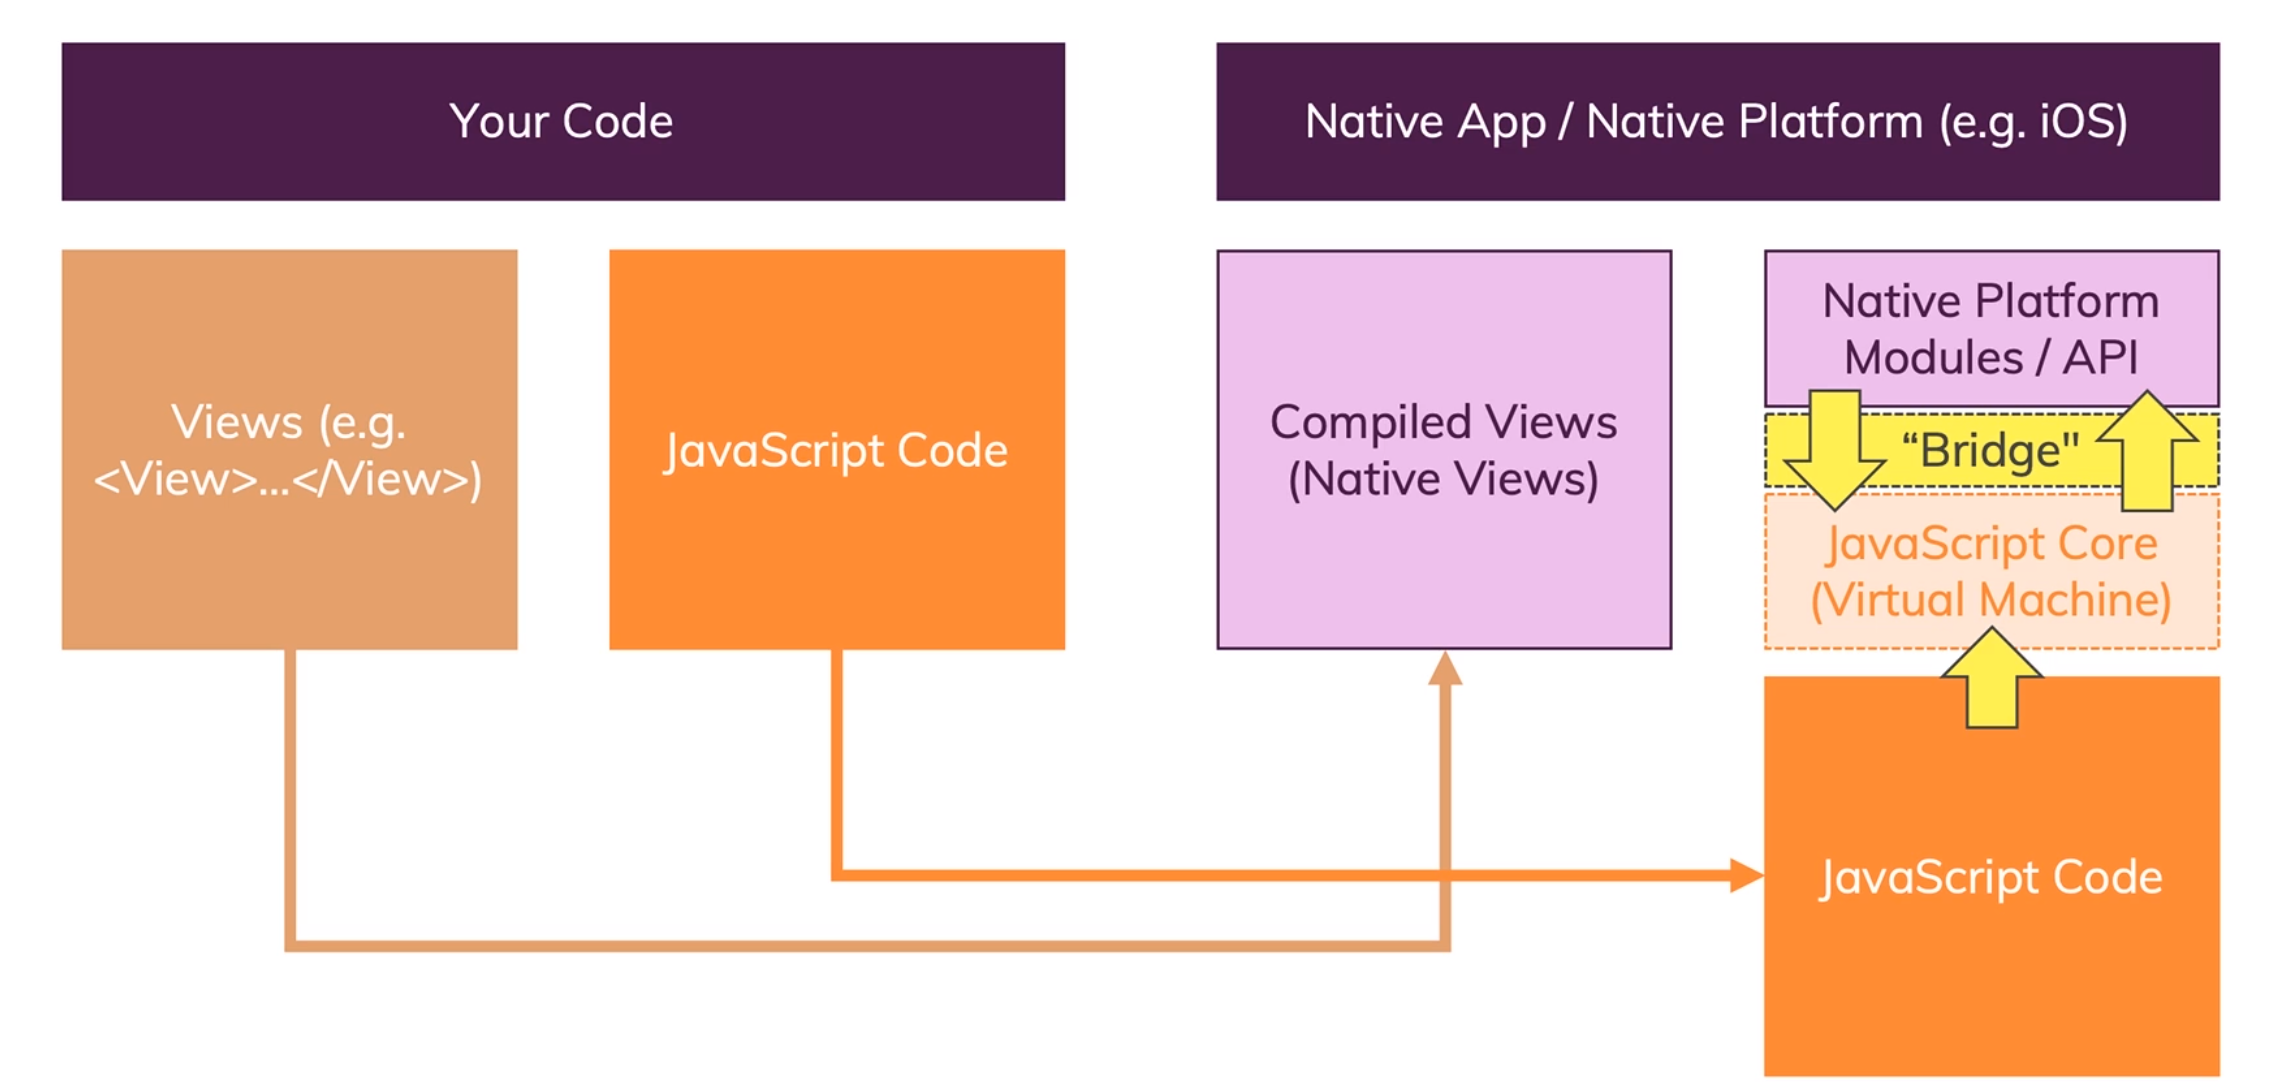
\includegraphics[height=6.5cm]{img/rn-working.png}}%
           {\scriptsize%
            Zdroj: \cite{udemy}}
	\caption{Ukážka fungovania React Native aplikácie}  
  \label{reactAppExplained}
\end{figure}
\subsubsection{Virtual \acrfull{dom}}
Ďalším dôležitým konceptom v React Native, je tzv. Virtual DOM. DOM je vo všeobecnosti skratka pre Document Object Model (inak nazývaný aj real DOM), čo je programové rozhranie pre \acrshort{html} a \acrshort{xml} dokumenty. DOM reprezentuje dokument ako skupinu uzlov (tzv. "nodes") a objektov. To umožňuje jazykom ako napríklad JavaScript modifikovať dané uzly a tým aj celý dokument. DOM je reprezentovaný ako dátový strom, vďaka čomu je každá zmena rýchla. Avšak po tejto zmene, elementy a ich potomkovia musia byť nanovo vyrenderované, aby nastala zmena aj priamo v \acrshort{ui} danej aplikácie. Proces renderovania je to, čo spôsobuje nezanedbateľné spomalenie výkonu, ktoré je navyše priamo úmerné so zväčšujúcim sa počtom \acrshort{ui} komponentov.

Tu prichádza na scénu Virtual DOM, ktorý dosahuje podstatne lepšie výsledky ako real DOM. Virtual DOM je iba virtuálne znázornenie DOM. Vždy, keď sa zmení stav aplikácie, namiesto real DOM sa aktualizuje virtual DOM. Akonáhle sa zmení stav ktoréhokoľvek elementu alebo sa vytvorí nový element, vytvorí sa spolu s ním aj nový virtual DOM. Následne prebehne proces porovnania (nazývaný "diffing") aktuálnej verzie a prechádzajúcej verzie vritual DOM. Potom sa vypočíta najlepší možný spôsob ako tieto zmeny premietnuť do real DOM. Akonáhle React vie, ktoré elementy vo virtual DOM boli zmenené, zaktualizuje len dané elementy v real DOM. Vďaka tomu je výkon neporovnateľne lepší v porovnaní s priamou manipuláciou s DOM. \cite{rn4}

\begin{figure}[!htbp]
  \centering  
  \def\stackalignment{c}
	\stackunder{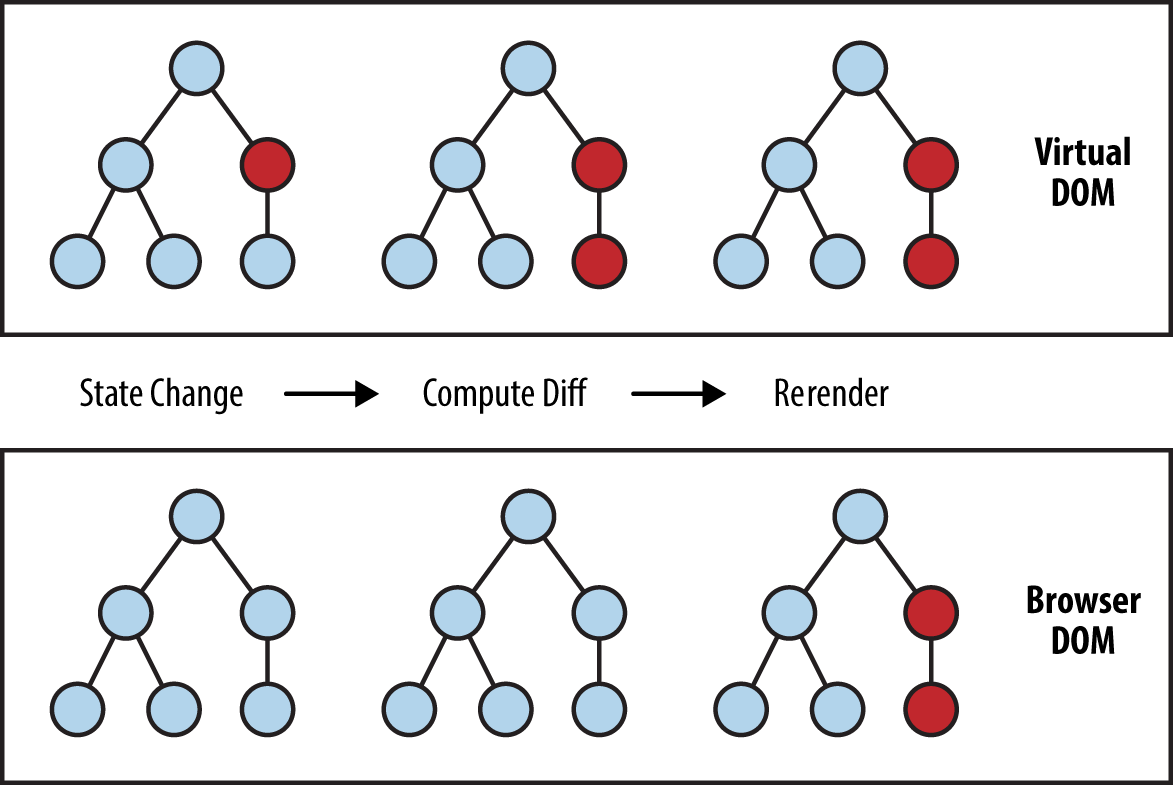
\includegraphics[width=12cm]{img/dom.png}}%
           {\scriptsize%
            Zdroj: \cite{oreily}}
	\caption{Virtual DOM vs. real DOM}  
  \label{domImg}
\end{figure}
Na \hyperref[domImg]{obrázku \ref{domImg}} vidíme červené kruhy, ktoré znázorňujú zmenené uzly. Tieto uzly reprezentujú konkrétne \acrshort{ui} elementy, ktoré zmenili svoj stav. Na hornej časti obrázku vidíme, že je najprv vypočítaný rozdiel medzi aktuálnou a predchádzajúcou verziou virtual DOM stromu, pričom celý podstrom rodiča je nanovo prerenderovaný a tým poskytne aktualizáciu \acrshort{ui}. Aktualizácie real DOM sa posielajú hromadne, namiesto odosielania aktualizácií pre každú jednu zmenu stavu, čo môžeme vidieť na dolnej časti obrázku. \\

\subsubsection{Základné komponenty}
Kľúčovým prvkom každej React Native aplikácie sú komponenty. Každý komponent má inú úlohu, no dokopy tvoria celok. Z hľadiska koncepcie môžeme povedať, že komponenty sú podobné JavaScript funkciám. Vedia prijímať vstupy (nazývané ``props''), s ktorými potom umožňujú pracovať vo vnútri komponentu a vracajú elementy, ktoré popisujú, čo sa má zobraziť na obrazovke. \cite{react}

V React Native existujú dva hlavné typy komponentov, ktoré tvoria aplikáciu.
\begin{itemize}[leftmargin=*]
{\bf \item Class komponenty} \newline
Sú to triedy rozširujúce základnú triedu z Reactu s názvom Component. Majú prístup k lifecycle metódam Reactu ako napríklad render či state/props funkcionalite od rodičovskej triedy. V súčasnosti sú menej používané kvôli tomu, že sú komplikovanejšie ako functional komponenty. Aj keď stále existujú prípady, v ktorých je ich syntax potrebná, vo všeobecnosti sa pri vytváraní nového komponentu viac používa syntax functional kompononetu. Vo \hyperref[classComponent]{výpise \ref{classComponent}} máme uvedený aj jednoduchý príklad class komponentu.  \\

\begin{lstlisting}[caption={Príklad class komponentu}, label={classComponent}]
import React, { Component } from 'react';
import { Text } from 'react-native';

class OurNewComponent extends Component {
  render() {
    return (
      <Text>This is our new class component</Text>
    );
  }
}

export default OurNewComponent;
\end{lstlisting}
{\bf \item Functional komponenty} \newline
Sú jednoduchší typ komponentu. Ich deklarácia je v podstate rovnaká ako pri obyčajnej JavaScript funkcii. V minulosti sa za ich nevýhodu oproti class komponentom považovalo to, že neumožňovali správu stavov (states) a nemali prístup k lifecycle metódam ktoré React Native poskytuje. To sa zmenilo až po vydaní verzie 16.8.0 v roku 2019, v ktorej vývojári pridali Hooks, čím tento problém zanikol. \cite{hooks} Odvtedy sa ich popularita ešte zvýšila a stali sa novým štandardom. Na \hyperref[funcComponent]{výpise \ref{funcComponent}} môžeme vidieť, že kód je celkovo jednoduchší a čitateľnejší, ako pri class komponentoch. \\

\begin{lstlisting}[caption={Príklad function komponentu}, label={funcComponent}]
import React from 'react';
import { Text } from 'react-native';

const OurNewComponent = () => {
  return (
    <Text>This is our new functional component</Text>
  );
}

export default OurNewComponent;
\end{lstlisting}

\end{itemize}

React Native navyše poskytuje aj sadu predpripravených hotových natívnych komponentov, ktoré sa dajú veľmi jednoducho použiť pri programovaní aplikácie. Patria medzi ne napríklad View, Text, Button, Image, či TextInput. \\

\subsubsection{Props a state}
Props a State sú dva typy dát, pomocou ktorých vieme pracovať s komponentami.
\begin{itemize}[leftmargin=*]
{\bf \item Props} \newline
Props (z anglického slova ``properties'') je obdoba argumentov pri klasických funkciách v JavaScripte alebo atribútov pri HTML. Komponenty prijímajú props od rodičovského komponentu. Ich dôležitou vlastnosťou je, že sú tzv. ``immutable'' tj. nemenné vo vnútri komponentu. V Reacte a v React Native smerujú dáta jedným smerom - od rodičovských komponentov k detským. Celý koncept props je založený na tom, že si viete vytvoriť jeden komponent, ktorý je možné použiť na viacerých miestach v aplikácii. Rodičovské komponenty potom vedia zavolať vami vytvorený komponent, pričom na rôznych miestach vie mať rozličné props. Props v zásade pomáhajú písať znovu použiteľný kód. \cite{props}
{\bf \item State} \newline
State pracuje odlišne v porovnaní s props. Je to interná vlastnosť komponentu, ktorá pomáha sledovať určité informácie. Použitím ``setState'' sa daný komponent a jeho detské komponenty nanovo vyrenderujú, vďaka čomu sa nemusí programátor zaoberať implementáciou event handlerov ako v iných jazykoch. State sa používa v situáciách, keď sa menia dáta v rámci komponentu. Dobrým príkladom je napríklad interakcia používateľa s komponentom, pri kliknutí na tlačidlo alebo zaškrtnutí checkboxu. Napríklad pri vypĺňaní formuláru má každý z textových inputov svoj vlastný state. Ak vyplníme daný input, automaticky sa mení jeho state, čo spôsobuje prerenderovanie celého komponentu a všetkých jeho detských komponentov. \cite{props} \\
\end{itemize} 
\subsubsection{Hooks}
Ich hlavnou úlohou je umožniť používať state a lifecycle metódy vo functional komponentoch, čo predtým bolo možné iba vytvorením class komponentov. Ich uvedenie výrazne zvýhodnilo používanie functional komponentov oproti class komponentom. Tak isto ako pri komponentoch, aj tu React Native umožňuje využiť predpripravené Hooks priamo od vývojárov. Najčastejšie používané sú useEffect a useState. V prípade potreby je možné si vytvoriť aj vlastný hook tak, aby spĺňal požadovanú funkcionalitu. \cite{hooks} \\
\subsection{Expo alebo React Native CLI ?}
Predtým ako sa programátor pustí do vývoja aplikácie pomocou React Native, ho čaká rozhodnutie či použiť pomocný framework Expo, alebo vstavanú funkcionalitu React Native CLI. Nato aby sme mohli vytvorenú aplikáciu vôbec spustiť, potrebujeme jednu z týchto technológii. \\

\subsubsection{Expo}
Framework používaný pri vytváraní React Native aplikácií. Je to balík nástrojov a služieb vytvorených pre React Native, ktoré zjednodušujú vývoj a deployment aplikácie na Android a iOS. \cite{expo} \newline

{\bf Výhody}
\begin{itemize}
{\item Nevyžaduje vedomosť programovania v natívnom kóde.}
{\item Nepoužíva Xcode alebo Android Studio.} 
{\item Najrýchlejší a najjednoduchší spôsob, ako vytvoriť natívne React Native aplikácie.}
{\item Uvoľňuje \acrshort{ota} updates.} 
{\item Vstavaný prístup k natívnym \acrshort{api}s} \cite{expo}
\end{itemize}

{\bf Nevýhody}
\begin{itemize}
{\item Ďalšia vrstva abstrakcie.} 
{\item Neumožňuje zasahovať do natívneho kódu.}
{\item Nie sú k dispozícií všetky iOS a Android \acrshort{api}s.} \cite{expo}
\end{itemize}
\bigskip

\subsubsection{React Native CLI}
Vstavaný nástroj v React Native, ktorý pomáha spustiť aplikáciu. \newline

{\bf Výhody}
\begin{itemize}
{\item Umožňuje zasahovať do natívneho kódu.} 
{\item Vieme pomocou neho pridávať natívne moduly (Objective C/Java).} \cite{rncli} 
\end{itemize}

{\bf Nevýhody}
\begin{itemize}
{\item Vývoj iOS aplikácie nie je možný na inom OS ako MacOS.} 
{\item Na vytvorenie projektu sa vyžaduje Android Studio alebo XCode.}
{\item Nastavenie projektu (vrátane konfigurácie) je pomerne komplikované a nepohodlné.} 
{\item Neposkytuje niektoré JavaScript \acrshort{api}s napr. push-notifikácie, je potrebné ich ručne doinštalovať.} \cite{rncli} \\
\end{itemize}

\subsubsection{Odôvodnenie výberu}
V našom prípade sme si vybrali pracovať s Expom, keďže práca s ním je jednoduchšia a priamočiarejšia a vzhľadom na typ a vlastnosti aplikácie, nám jeho funkcionalita plne postačuje. \\

\subsection{Node.js}
Ako technológiu pre backend sme zvolili Node.js, čo je open-source, cross-platformové, back-endové runtime prostredie JavaScriptu, ktoré beží na Chrome V8 JavaScript engine a vykonáva kód JavaScript mimo webového prehliadača. \cite{nodejswiki} Tento engine prekladá JavaScriptový kód do rýchlejšieho strojového kódu. Vznik Node.js bol logickým krokom po tom, ako vývojári JavaScriptu rozšírili použiteľnosť jazyka z čisto skriptovacieho, ktorý bolo možné používať a spúšťať iba v prehliadači, na jazyk ktorý umožňuje vytvoriť samostatnú aplikáciu spustiteľnú aj mimo prehliadača. 

Nesporným prínosom node.js je, že využíva tzv. event-driven non-blocking I/O model, ktorý ho robí efektívnym. I/O alebo aj input/output, môže byť čokoľvek od čítania resp. zapisovania lokálnych súborov, až po vytváranie \acrshort{http} requestov na \acrshort{api}. Non - blocking znamená, že aktuálne vykonávaný request neblokuje spustenie ďalšieho requestu počas čakania na odpoveď. Na \hyperref[nodejsImg]{ obrázku \ref{nodejsImg}} nižšie môžeme vidieť porovnanie blocking (vľavo) a non blocking modelu (vpravo) na príklade s databázou. \cite{nodejs} \\

\begin{figure}[!htbp]
  \centering  
  \def\stackalignment{c}
	\stackunder{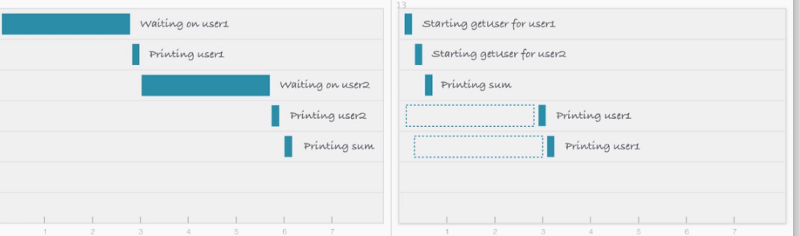
\includegraphics[width=16cm]{img/nodejs.png}}%
           {\scriptsize%
            Zdroj: \cite{nodejs}}
	\caption{Porovnanie blocking a non-blocking modelu}  
  \label{nodejsImg}
\end{figure}

\subsubsection{Yarn}
Je package manager pre JavaScript, ktorý pomáha riadiť dodatočne doinštalované knižnice a rôzne iné dependencies v našom projekte. Keďže v súčasnej dobe sa pri programovaní využíva veľké množstvo knižníc a závislosti, aby sa zjednodušila práca programátora a nemusel istú funkcionalitu programovať nanovo, je odporúčané package manager používať.

Node.js prichádza s predinštalovaným package managerom npm. Napriek tomu sme sa rozhodli použiť yarn, ktorý bol vytvorený Facebookom, tak isto ako React Native a preto práca s ním bola konzistentnejšia a bez väčších problémov na rozdiel od npm. \\

\subsubsection{Axios}
Axios je knižnica pre JavaScript, ktorá sa používa na vytváranie \acrshort{http} requestov z Node.js alebo XML HttpRequests z prehliadača. Podporuje aj \acrshort{es6} promise \acrshort{api}, pričom ešte viac uľahčuje celý proces okolo requestov tým, že ešte viac zlepšila dobre fungujúcu fetch() funckiu z JS a vylepšila error handling. \cite{axios} \\

\subsection{The Movie Database}
 \acrfull{tmdb}, je databáza filmov a TV seriálov, ktorá bola vytvorená v roku 2008 úzkou komunitou ľudí, ktorá sa neskôr postupne rozrástla. Dnes je TMDb používaná vyše 400 000 developermi a firmami. \cite{tmdb} Úspech im priniesla hlavne ich dostupná \acrshort{api}, ktorá je zadarmo a ponúka širokú škálu queries, pomocou ktorých je možné získať podrobné informácie o filmových tituloch. Ich veľkou prednosťou je aj množstvo dostupných titulných plagátov k filmom vo vysokej kvalite. Jedinou jej nevýhodou je, že popularitou zatiaľ nedosahuje úroveň najväčšej databázy na svete \acrshort{imdb} a pri niektorých filmoch nie sú ich hodnotenia kredibilné. \\

\subsection{Firebase}
Firebase je platforma vyvinutá spoločnosťou Google, ktorá pomáha vytvárať, zlepšovať a rozširovať funkcionalitu aplikácií. Obsahuje sadu nástrojov, ktoré pokrývajú veľkú časť služieb, ktoré by si vývojári museli inak sami naprogramovať. Patria sem napríklad analytika, autentifikácia používateľov, databázy, konfigurácia, ukladanie súborov, doručovanie push notifikácií a mnoho iného. Služby sú uložené v cloude a sú škálovateľné s malým resp. minimálnym úsilím zo strany vývojára. \cite{firebase} \\

\subsubsection{Firebase authentication}
\label{sec:firebaseauth}
Poskytuje backendové služby, jednoducho použiteľné \acrshort{sdk} a predpripravené \acrshort{ui} knižnice na autentifikáciu používateľov v aplikácii. Podporuje autentifikáciu pomocou hesla, telefónneho čísla, Googlu, Facebooku a Twitteru. Je úzko integrovaná s ostatnými službami Firebase a využíva  štandardy ako OAuth 2.0 a OpenID Connect, takže ju možno ľahko integrovať do vlastného backendu. \cite{auth} Okrem autentifikácie umožňuje aj registráciu a správu zaregistrovaných používateľov. V našej aplikácií sme si zvolili použiť autentifikáciu pomocou emailu a hesla. \\

\subsubsection{Cloud Firestore}
\label{sec:firestore}
Je škálovateľná NoSQL cloudová databáza, pre vývoj mobilných a webových aplikácii. Udržuje dáta synchronizované medzi klientskými aplikáciami prostredníctvom listenerov v reálnom čase.

Vo Firestore dátovom modeli \hyperref[firestore]{(pozri obr. \ref{firestore})}, sa dáta ukladajú do tzv. dokumentov, ktoré obsahujú polia (fields) namapované na konkrétne hodnoty. Tieto dokumenty sú ukladané do kolekcií, ktoré slúžia ako kontainer pre viacero dokumentov. Dokumenty podporujú mnoho rôznych dátových typov, od jednoduchých ako sú napríklad reťazce alebo čísla, až po komplexnejšie ako mapy, polia, alebo vnorené objekty. \cite{firestoredoc}

Friebase ponúka aj druhý typ databázy, Firebase Realtime Database, čo je tiež NoSQL cloudová databáza. Oproti Firestore ponúka jednoduchší dátový model, v ktorom sa dáta ukladajú iba vo formáte \acrshort{json}, čo je vhodné iba pri jednoduchšej dátovej štruktúre. Taktiež nepodporuje používanie zložitejších queries. Firestore bol teda v našom prípade lepšou voľbou. \\

\begin{figure}[!htbp]
  \centering  
  \def\stackalignment{c}
	\stackunder{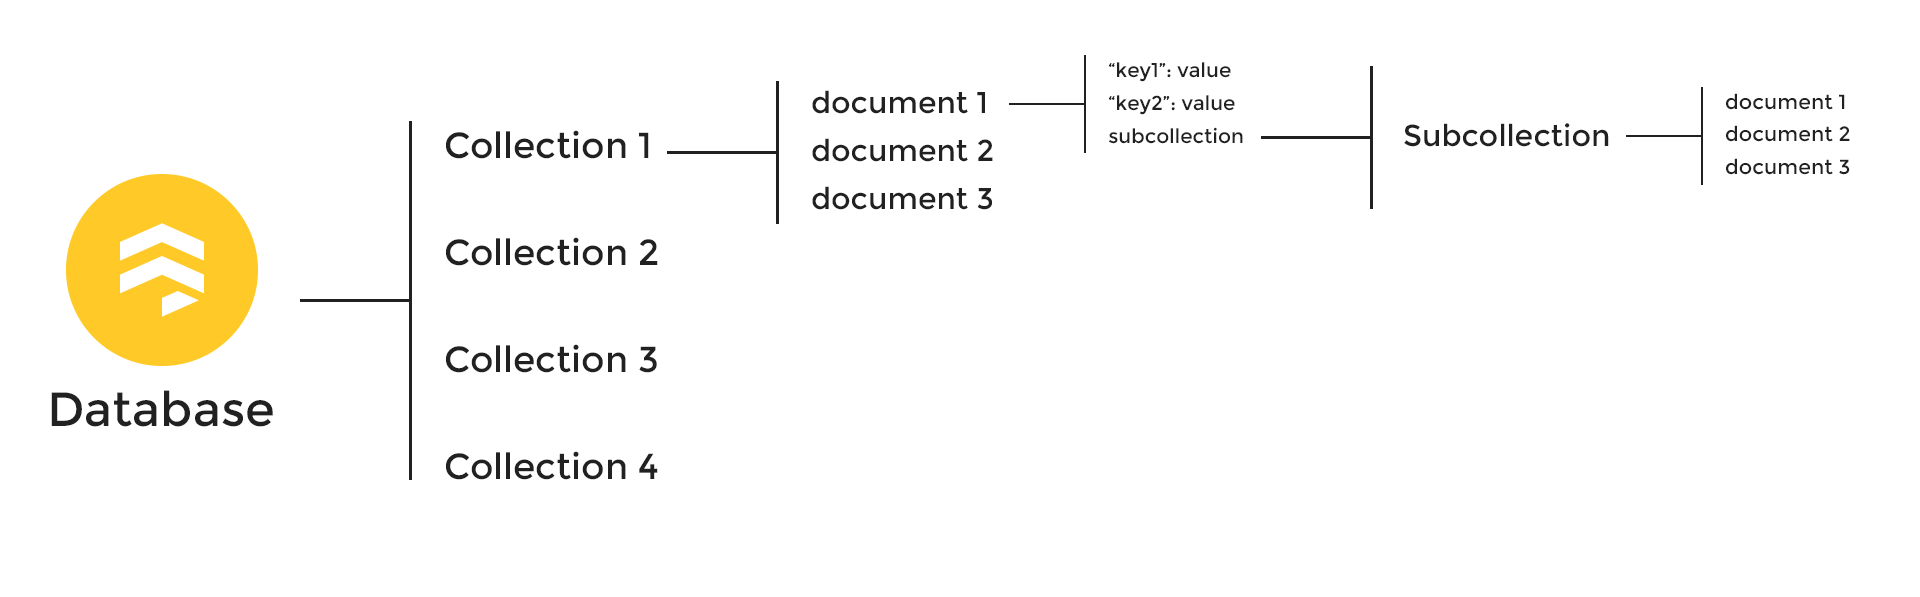
\includegraphics[width=15cm]{img/firestore.png}}%
           {\scriptsize%
            Zdroj: \cite{firestoreimg}}
	\caption{Znázornenie dátového modelu Cloud Firestore} 
  \label{firestore}
\end{figure}


\section{Analytická a návrh systému}
\subsection{Analýza problému}
V dnešnej dobe, kedy je ponuka produktov na trhu veľmi veľká a pestrá, býva častým problémom používateľov nájsť práve tie produkty o ktoré majú reálne záujem a vyhovujú ich kritériám. Práve tento problém bol motiváciou pre vznik odporúčacích systémov \hyperref[sec:odporucacie systemy]{(kapitola 1.1)}, ktoré sa dnes vo veľkej miere využívajú. 

Jedným z prípadov, pri ktorom sa s daným problémom často stretávame, je výber filmového titulu. S príchodom streamovacích služieb ako Netflix, Amazon Prime, Hulu či HBO GO, vďaka ktorým sú dostupné milióny titulov, je veľmi náročné vybrať si tie, ktoré budú vyhovovať osobným preferenciám jednotlivca. Väčšina spoločností to vyriešila zavedením odporúčacích systémov a používaním rôznych rebríčkov popularity. To však vyriešilo iba situáciu, ak sa človek rozhodne pozerať film sám. Bežne sa však stáva, že ľudia chcú pozerať film vo dvojici a pri spoločnom výbere filmu strávia neprimerane veľa času prezeraním rôznych filmových databáz a rebríčkov filmov. 

To nám vnuklo myšlienku, na tému tejto bakalárskej práce s cieľom zjednodušiť výber filmu  prostredníctvom mobilnej aplikácie, založenej na odporúčacích systémoch.

\subsection{Existujúce riešenia problému}
Pri analýze súčasného stavu sme sa pozreli na existujúce riešenia, venujúce sa danej problematike. Je dôležité poznamenať, že v čase zadania práce nebola dostupná aplikácia, ktorá by obsahovala podobnú funkcionalitu a bola by dostupná na oba spomínané operačné systémy. 
\subsubsection{Android OS}
Na OS Android bola dostupná len jedna aplikácia vytvorená v roku 2019, avšak už dlhšie nepodporovaná vývojárom. Aplikácia s názvom MovieMatch má však viacero nevýhod oproti riešeniu, ktoré sme navrhli my. Základným prvkom tejto aplikácie je skupina, kým v žiadnej nie ste, nemáte možnosť si prezerať a hodnotiť filmové tituly. Po nainštalovaní a spustení, vygeneruje aplikácia kód, ktorý treba poslať iným používateľom, aby sa mohli pripojiť do jeho skupiny. Tak isto sa používateľ vie pripojiť do inej skupiny pomocou kódu danej skupiny. Toto riešenie spôsobuje, že používateľ je závislý od iných používateľov a bez nich je aplikácia nepoužiteľná. Nevýhodou je aj spôsob implementácie, vo forme webovej aplikácie, ktorá sa otvára priamo v prehliadači. To vzhľadom na súčasné štandardy vývoja mobilných aplikácií nie je najvhodnejšie riešenie a \acrshort{ui} oproti natívnym a hybridným (resp. cross platformovým) aplikáciám pôsobí zastaralo. Detailnému porovnaniu typov mobilných aplikácií sme sa venovali v \hyperref[sec:typy aplikacii]{kapitole 1.2.}
\subsubsection{iOS}
V čase zadania tejto bakalárskej práce nebola podobná aplikácia bežiaca na operačnom systéme iOS k dispozícií. To sa neskôr zmenilo, keď v novembri 2020 vyšla aplikácia Movie Match. Funkcionalitou a vzhľadom je na tom omnoho lepšie ako spomínaná Android aplikácia. Z jej používania však nie je jasné, či pri generovaní filmov využíva nejaký druh odporúčacieho algoritmu, alebo generuje filmy každému používateľovi rovnako. To ma za následok, že  používateľ nenadobudne pocit, že sa aplikácia časom prispôsobuje jeho preferenciám. 


\subsection{Návrh riešenia}
Cieľom tejto bakalárskej práce bolo navrhnúť a implementovať mobilnú aplikáciu, ktorá bude slúžiť ako pomocník pri spoločnom výbere filmu dvoch používateľov. Na základe ich osobného profilu preferencií jednotlivých atribútov filmov, sa im vygenerujú odporúčané filmy, ktoré budú môcť obaja hodnotiť a následne si pozrieť zhodu. Používateľ bude vedieť hodnotiť filmy aj samostatne bez nutnosti byť prepojený s iným používateľom. Hodnotenie filmov bude vo forme binárneho hodnotenia (like/dislike) a implementované pomocou známeho swipeovania na obrazovke doprava a doľava. Na základe týchto hodnotení sa mu budú meniť preferencie a následne aj odporúčané tituly. Celý tento princíp obsahuje prvky content based filteringu, čo je jedna z metód odporúčacích systémov \hyperref[sec:contentbased]{(kapitola 1.1.6).}

V rámci implementácie, sme sa rozhodli, aby aplikácia fungovala pre oba populárne operačné systémy (Android aj iOS), vďaka čomu používatelia nebudú obmedzovaní a viazaní na jeden operačný systém. Zvolením frameworku React Native sme teda zabezpečili vytvorenie cross platformovej aplikácie. Sústredili sme sa prioritne na OS Android, avšak po malých dodatočných úpravách, by v budúcnosti nemal byť problém aplikáciu spustiť aj na iOS. Autentifikácia používateľa je formou emailu a hesla implementovaná pomocou Firebase authentication. Ako úložisko dát nám slúži cloudová NoSQL databáza Firestore. Ako zdroj filmových dát sme zvolili databázu TMDb, pričom na prácu s dátami sme využívali ich \acrshort{api}. 
\vspace{55mm} %5mm vertical space

\begin{figure}[hbt!]
  \centering  
  \def\stackalignment{c}
	\stackunder{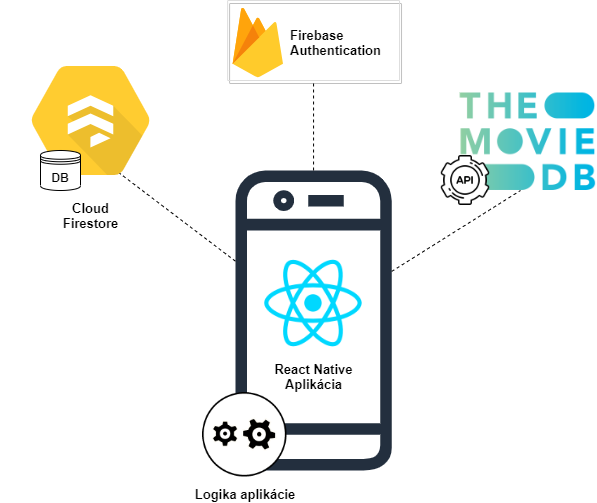
\includegraphics[height=10cm]{img/app-diagram.png}}%
           {\scriptsize}
	\caption{Znázornenie konceptu aplikácie}  
  \label{app-diagram}
\end{figure}

V ďalšej časti práce je návrh detailnejšie vizualizovaný pomocou vybraných UML diagramov. 

\pagebreak

\subsubsection{Diagramy prípadov použitia}
\begin{figure}[hbt!]
  \centering  
  \def\stackalignment{c}
	\stackunder{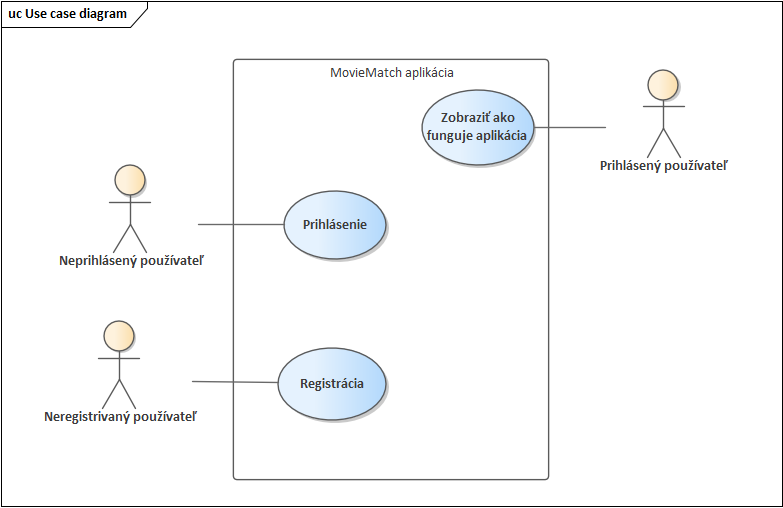
\includegraphics[height=10cm]{img/usecase1.png}}%
           {\scriptsize}
	\caption{Diagram prípadov použitia 1}
	\label{usecase1}
\end{figure}

Na \hyperref[usecase1]{obrázku \ref{usecase1}} môžeme vidieť, že aplikácia rozlišuje 3 základné role a to neregistrovaný používateľ a registrovaný resp. prihlásený používateľ. Neregistrovaný používateľ sa vie zaregistrovať pomocou zvolenej prezývky, emailu a hesla. Následne ho aplikácia rovno prihlási pričom mu zobrazí krátky návod na oboznámenie sa s aplikáciou. Na jeho konci je z populárnych titulov vygenerovaný úvodný dotazník, v ktorom je požívateľ vyzvaný, aby pomocou swipeovania vybral aspoň 15 filmových titulov ktoré sa mu páčia. To zabezpečí, že sa profil preferencií inicializuje. Registrovaný používateľ sa vie prihlásiť pomocou emailu a hesla.
\pagebreak

\begin{figure}[hbt!]
  \centering  
  \def\stackalignment{c}
	\stackunder{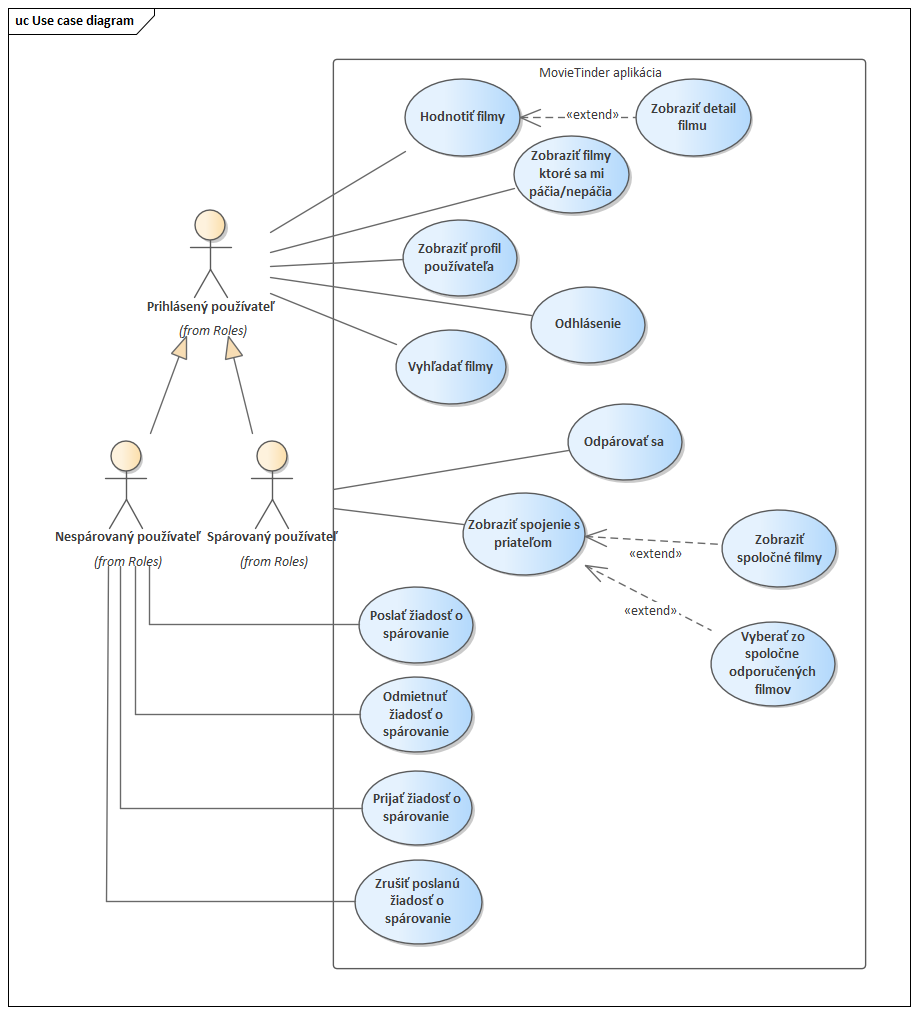
\includegraphics[width=15cm]{img/usecase2.png}}%
           {\scriptsize}
	\caption{Diagram prípadov použitia 2}
  \label{usecase2}
\end{figure}
Na \hyperref[usecase2]{obrázku \ref{usecase2}} máme detailnejší popis aplikácie po prihlásení používateľa. Prihlásený používateľ má možnosť hodnotiť filmy, prípadne si pozrieť detail aktuálne zobrazeného filmu. Tak isto si vie zobraziť svoju knižnicu, v ktorej má ohodnotené filmy. Vie si tiež zobraziť svoj profil so základnými informáciami o jeho účte a odhlásiť sa z aplikácie. Po prihlásení môže používateľ nadobudnúť dve ďalšie podrole. 

Nespárovaný používateľ vie poslať žiadosť o spárovanie inému používateľovi, ktorú v prípade neobdržania odpovede vie kedykoľvek zrušiť. Vďaka tomu sa vyhne situácií, kedy by sa zasekol v stave čakania na odpoveď. Po obdržaní takejto žiadosti, vie túto žiadosť odmietnuť alebo prijať. Prijatím sa automaticky spáruje s druhým používateľom a na základe ich profilov preferencií sa im vygenerujú spoločné odporúčané filmové tituly, ktoré vedia obaja používatelia hodnotiť. 

Každý spárovaný používateľ má možnosť si pozrieť aktuálne spojenie, hodnotiť v ňom filmy, pozerať si spoločné zhody a v neposlednom rade má možnosť sa odpárovať a následne spárovať s ďalším používateľom. 

\subsubsection{Diagram tried}
\begin{figure}[hbt!]
  \centering  
  \def\stackalignment{c}
	\stackunder{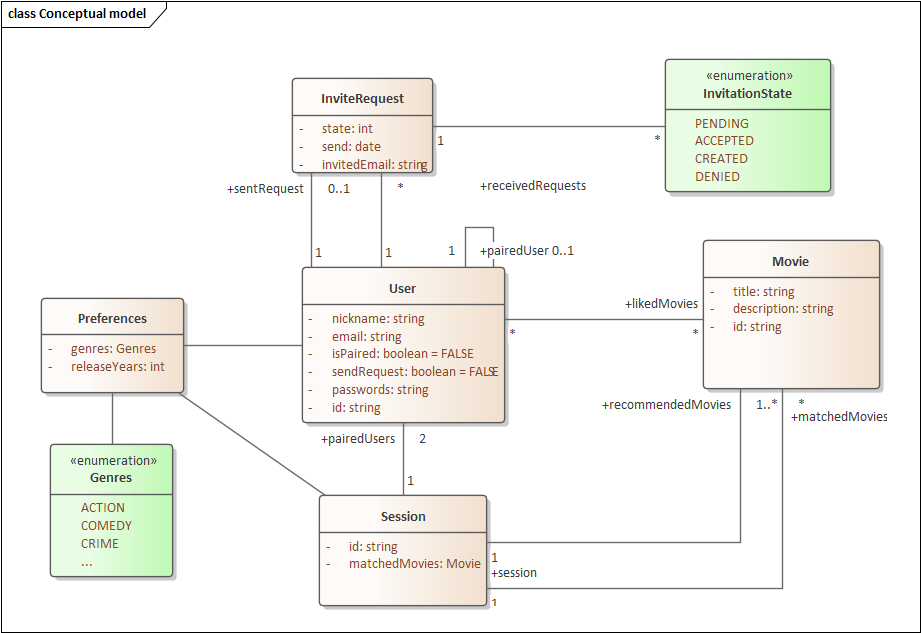
\includegraphics[width=15cm]{img/conceptualmodel.png}}%
           {\scriptsize}
	\caption{UML diagram tried}  
  \label{classdiagram}
\end{figure}
\hyperref[classdiagram]{Obrázok 10} zobrazuje diagram tried aplikácie. Ústredným prvkom našej aplikácie je trieda User, ktorá reprezentuje používateľov tohto systému. Používateľ vie byť v spojení s najviac jedným ďalším používateľom pomocou triedy Session. Táto trieda predstavuje spojenie medzi dvoma používateľmi a na základe preferencií, ktoré majú používatelia, sa v tomto spojení generujú odporúčané filmové tituly. Okrem toho je možné si v danom spojení pozrieť filmy, ktoré obaja používatelia hodnotili pozitívne. Samotný používateľ má vlastné spojenie s triedou Movie, vďaka ktorému si vie zobraziť filmy, ktoré sa mu páčili.

Každý používateľ vie obdržať viacero pozvánok na spojenie, ktoré sú reprezentované triedou InviteRequest, avšak prijať vie práve jednu. Odoslať vie tak isto iba jednu, čo zabraňuje situácii, kedy by viacero používateľov prijalo pozvánku jedného používateľa. Po odoslaní je pozvánka v stave pending kým na ňu príjemca neodpovie. Po prijatí pozvánky sa medzi používateľmi vytvorí spojenie, v ktorom si spolu vyberajú filmové tituly až kým sa nerozhodnú toto spojenie ukončiť. Trieda Preferences je dôležitým prvkom v systéme odporúčaní, keďže pomocou nej sa generujú odporúčané tituly pre jednotlivé spojenia.

%Význam väčšiny atribútov je z ich názvu jasný, preto spomenieme len tie, ktoré považujeme za potrebné objasniť. Pri triede User atribút isPaired vyjadruje, či daný používateľ je spárovaný s iným používateľom a atribút sendRequest, či daný používateľ poslal žiadosť o spárovanie inému používateľovi. 

\section{Implementačná časť}
V tejto časti práce sa pozrieme na celý implementačný proces od úvodného nastavenia a inštalácie potrebných nástrojov, až po konkrétne časti implementácie aplikácie.

\subsection{Úvodná inštalácia a nastavenia}
Predtým ako sme začali s programovaním aplikácie, bolo treba nastaviť a nainštalovať potrebné nástroje.
\subsubsection{VSCode}
Ako vývojové prostredie sme si vybrali Visual Studio Code. Výber vychádzal hlavne z osobných preferencií a dostupnosti množstva užitočných rozšírení. Stiahli sme ho z \href{https://code.visualstudio.com/download}{oficiálnej stránky} vývojára.
\subsubsection{React Native}
\begin{itemize}
{\item Ako prvé bolo treba nainštalovať Node.js z jeho \href{https://nodejs.org/en/download/}{oficiálnej stránky}. Kvôli stabilite sme stiahli LTS verziu. Inštalácia obsahuje aj predvolený package manager npm.} 
{\item Keďže sme počas implementácie uprednostnili yarn namiesto npm, bolo ho treba najprv doinštalovať pomocou npm príkazu \textit{npm install -g yarn}.} 
{\item Potom sme pomocou yarnu a príkazu \textit{yarn global add expo-cli}, nainštalovali Expo CLI.} 
{\item Posledným krokom k úspešnému spusteniu aplikácie je nainštalovanie emulátora, ktorý bude slúžiť ako virtuálne prostredie pre spustenie našej aplikácie počas programovania. Expo CLI síce podporuje aj spustenie na reálnom zariadení, emulátor je však pohodlnejšie riešenie. V našom prípade, keďže sme aplikáciu programovali primárne pre Android OS, nám nato poslúži \href{https://developer.android.com/studio}{Android Studio}, ktoré túto funkcionalitu obsahuje.}
\end{itemize}

\subsubsection{Firebase}
Na využitie Firebase bolo potrebné sa prihlásiť, založiť si nový projekt a napojiť ho na našu aplikáciu. Po zadaní povinných údajov, sa nám vygeneruje objekt s konfiguračnými údajmi. Ten si skopírujeme a vložíme do novovytvoreného súboru v našej aplikácií s názvom keys.js. Tam budeme uchovávať všetky potrebné citlivé údaje ako napríklad \acrshort{api} kľúče a podobne.

Posledným krokom inštalácie je pridanie firebase cez yarn príkazom \textit{yarn add firebase} a následné pridanie inicializácie v hlavnom súbore App.js pridaním funkcie \textit{firebase.initializeApp(config)}, kde argumentom je spomínaný konfiguračný objekt.
\subsubsection{Firebase authentication}
Firebase ponúka mnoho rôznych spôsobov autentifikácie používateľa. My sme zvolili klasický pomocou emailu a hesla. Vo firebase console sme v záložke authentication povolili metódu prihlasovania email/password. 
\subsubsection{\acrshort{tmdb}}
Na využívanie databázy filmových titulov \acrshort{tmdb} resp. jej \acrshort{api}, bolo potrebné si na web stránke služby založiť účet. Následne nám bol vygenerovaný \acrshort{api} kľúč, ktorý sme vložili do spomínaného súboru keys.js. 
\subsubsection{GitHub}
Na zálohovanie zdrojového kódu sme použili \href{https://github.com/}{GitHub}, voľne dostupnú webovú službu, ktorá poskytuje zálohu kódu, jeho verzionovanie prípadne sledovanie zmien a mnohé iné užitočné funkcie. Je jednou z najpopulárnejších služieb s týmto zameraním. Repozitár s našou aplikáciou je zverejnený na odkaze na \hyperref[ghqrcode]{obrázku \ref{ghqrcode}}. 

\begin{figure}[hbt!]
  \centering   
  \def\stackalignment{c}
	\stackunder{
\includegraphics[height=5cm]{img/github_qr.png}}%
           {\scriptsize%
            \url{https://github.com/adamt1312/MovieMatchApp}}
	\caption{QR kód GitHub repozitára aplikácie}  
  \label{ghqrcode}
\end{figure}
\subsection{Súborová štruktúra aplikácie}
V koreňovom adresári aplikácie máme hlavný súbor aplikácie App.js, kde načítavame použité fonty, pozadia a inicializujeme Firebase. Ďalšie dva podpriečinky \textit{src} a \textit{navigation} uchovávajú zvyšný zdrojový kód. 

Priečinok \textit{src} obsahuje nasledujúce podpriečinky:
\begin{itemize}
{\item \textbf{API} - zahŕňa súbory týkajúce sa Firebase a práce s databázou Firestore} 
{\item \textbf{assets} - uchováva všetky použité fonty, obrázky a ikony} 
{\item \textbf{components} - združuje všetky nami vytvorené komponenty} 
{\item \textbf{screens} - obsahuje všetky obrazovky a ich štýlovania}
\end{itemize}

Priečinok \textit{navigation} pozostáva z rôznych druhov navigácií, ktorým sa budeme venovať v \hyperref[sec:screens]{ďalšej časti} implementácie.

\subsection{Obrazovky v aplikácií}
\label{sec:screens}
Keďže sme v aplikácií použili viacero obrazoviek, bolo treba ich vytvoriť a vhodným spôsobom prepojiť tak, aby sa medzi nimi dalo navzájom pohybovať. Vytvorenie logického a intuitívneho ovládania, je dôležitým prvkom pri implementácií mobilnej aplikácie.
\subsubsection{React Navigation}
Nato aby sa dalo v React Native pohybovať medzi rôznymi obrazovkami slúži knižnica React Navigation. Pridali sme ju pomocou príkazu \textit{yarn add react-navigation}. Tak isto sme vždy pridali aj konkrétne druhy navigácií ktoré sme neskôr použili.
\subsubsection{Stack navigator}
Základná navigácia, ktorá umožňuje presúvanie medzi obrazovkami je stack navigator. Po jej vytvorení sme ju použili ako detský komponent v nami vytvorenom komponente MainStackNavigator. 

Keďže stack navigator slúži ako kontajner, popridávali sme doňho všetky ostatné typy navigácií s vlastnými obrazovkami a obrazovky, ktoré nie sú v žiadnej konkrétnej navigácií. Obrazovka ktorá bude v stack navigatore ako prvá v poradí, sa aj reálne vyrenderuje ako prvá pri spustení aplikácie. 

\subsubsection{Drawer navigation}
Drawer navigation je typ navigácie, ktorý pôsobí ako menu, ktoré sa dá otvoriť potiahnutím do strany na obrazovke. Do tejto navigácie sme vložili obrazovky Home, MyProfile a Requests (obrazovku žiadostí o spojenie). Pomocou tejto navigácie sme umožnili aj odhlásenie používateľa.
\subsubsection{Tab navigation}
Tab navigation slúži na prepínanie medzi viacerými obrazovkami v spodnej lište. Použili sme 3 takéto navigácie s rôznymi obrazovkami: 
\begin{itemize}
{\item Prvá obsahuje obrazovku ExploreMovies na objavovanie filmov a obrazovku FindFriend, ktorá slúži na vyhľadanie partnera na spoločné pozeranie. } 
{\item Druhá predstavuje používateľovu knižnicu, pričom združuje obrazovky LikedMovies a DislikedMovies.} 
{\item Posledná je použitá pri zobrazení spojenia dvoch používateľov, kedy zobrazuje obrazovku RecommendedMovies s odporučenými filmami pre dané spojenie a MatchedMovies, ktorý zobrazí filmy, ktoré sa páčili obom používateľom.} 
\end{itemize}

Na \hyperref[tabnav]{obrázku \ref{tabnav}} sú zobrazené všetky 3 tab navigácie po vložení konkrétnych obrazoviek.

\begin{figure}[hbt!]
  \centering   
  \def\stackalignment{c}
	\stackunder{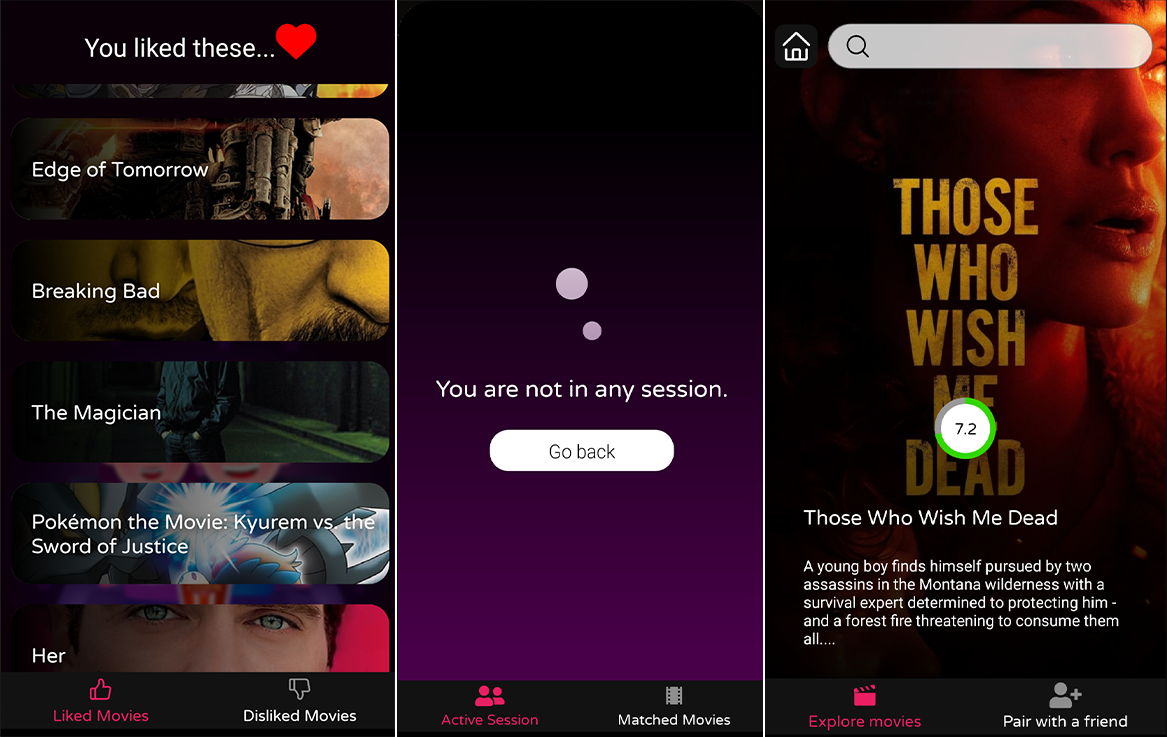
\includegraphics[width=15cm]{img/tabnav.png}}%
           \scriptsize
	\caption{Ukážka tab navigácií}  
  \label{tabnav}
\end{figure}

\subsection{Autentifikácia používateľa}
Ďalšou dôležitou súčasťou aplikácie je autentifikácia používateľov.

Našou úlohou bolo použiť dostupné funkcie od Firebase na registráciu a prihlásenie a doručiť im registračné resp. prihlasovacie údaje zadané používateľom. Následne sme vytvorili komponent v ktorom sme implementovali jednoduchú logiku zobrazovania obrazoviek, v závislosti od toho, či je používateľ prihlásený alebo sa práve zaregistroval.
\subsubsection{Registrácia}
Na registráciu sme vytvorili vlastnú funkciu \textit{registration}, ktorá vykoná všetko potrebné. Najprv sa zavolá asynchrónna funkcia \textit{firebase.auth().createUserWithEmailAndPassword(email, password)}, ktorá vytvorí účet s danými údajmi ak ešte neexistuje. Následne si používateľa vytvoríme aj v databáze Firestore. 
\subsubsection{Prihlásenie a odhlásenie}
Prihlasovanie rieši naša vlastná funkcia \textit{signIn}, v ktorej sa volá asynchrónna funkcia \textit{firebase.auth().signInWithEmailAndPassword(email,password)} od firebase. 

Odhlásenie bolo implementované jednoducho pomocou funkcie \textit{firebase.auth().signOut()}.
\subsubsection{Dokončenie logiky}
Nato aby aplikácia vedela akú obrazovku má po otvorení zobraziť sme vytvorili komponent Loading, ktorý sme vložili do stack navigatoru ako prvú obrazovku v poradí. Tento komponent zobrazuje načítavanie pri spustení aplikácie a zároveň vo vnútri obsahuje jednoduchú rozhodovaciu logiku, či zobraziť domácu obrazovku pre prihláseného používateľa, alebo prihlasovaciu obrazovku. 

To sme docielili pomocou nastavenia pozorovateľa na authentication stav vďaka asynchrónnej funkcii \textit{firebase.auth().onAuthStateChanged()}, ktorá sa spustí pri zmene daného stavu. Jednoducho povedané, spustí sa vždy, keď sa používateľ odhlási, prihlási alebo zaregistruje, pričom vráti buď objekt používateľa alebo null. V prípade vrátenia null, aplikácia zobrazí prihlasovaciu obrazovku. Ak funkcia vráti používateľa, skontrolujeme či sa práve zaregistroval, aby sme vedeli či je potrebné mu zobraziť návod na použitie aplikácie a úvodný dotazník. Pokiaľ to nie je nový používateľ, aplikácia mu rovno zobrazí domácu obrazovku. 
\subsection{Štruktúra databázy}
Na ukladanie údajov sme použili NoSQL cloud databázu Firestore. Tá obsahuje dve základné kolekcie \textit{Users} a  \textit{Sessions}. 

Kolekcia \textit{Users} združuje všetkých používateľov vo forme jednotlivých dokumentov, ktorých názov je unikátne id daného používateľa. Obsah jednotlivých dokumentov tvoria základné informácie o používateľovi. Dôležité pre proces párovania budú hlavne položky \textit{isPaired} a \textit{sentRequest}. Prvá z nich môže mať buď hodnotu null alebo id spojenia v ktorom používateľ figuruje. Druhá môže mať taktiež null alebo id používateľa ktorému bola odoslaná žiadosť o spojenie. Dokument obsahuje aj ďalšie subkolekcie dokumentov a to kolekcie pozitívne a negatívne ohodnotených filmov, kolekciu čakajúcich žiadosti o spojenie a kolekciu preferencií používateľa.

Kolekcia \textit{Sessions} obsahuje jednotlivé spojenia taktiež vo forme dokumentov. Dokument zahŕňa id oboch používateľov, id filmov ktoré používatelia označili, že sa im páčia a preferencie daného spojenia vygenerované na základe preferencií oboch používateľov. Spojenie ďalej zahŕňa subkolekciu odporúčaných filmov daného spojenia. 
\vspace{55mm}

\begin{figure}[hbt!]
  \centering   
  \def\stackalignment{c}
	\stackunder{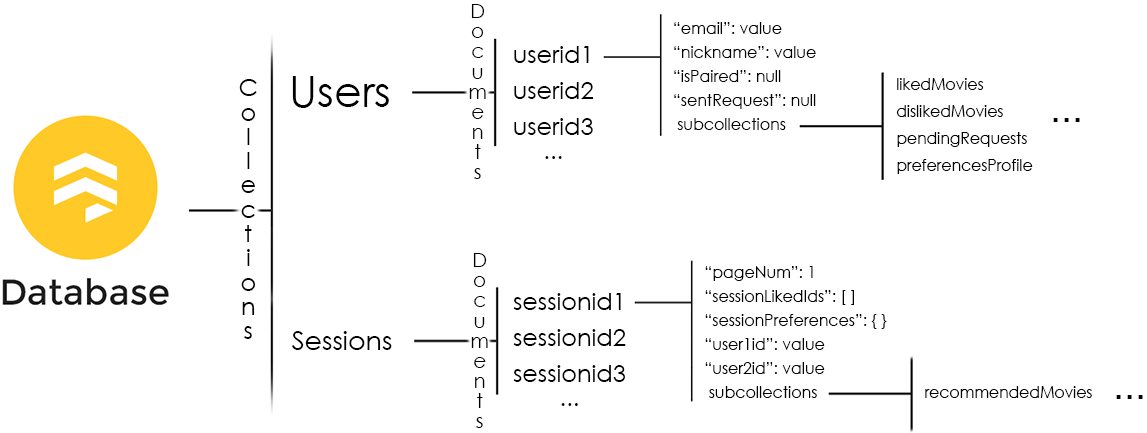
\includegraphics[width=16cm]{img/db_structure.png}}%
           \scriptsize
	\caption{Firestore štruktúra}  
  \label{dbstructure}
\end{figure}

\subsection{Mechanizmus párovania}
Keďže medzi hlavné vlastnosti aplikácie patrí možnosť spárovania dvoch používateľov, bolo potrebné naprogramovať kompletnú logiku okolo tohto procesu. 

Ako sme spomenuli v predchádzajúcej kapitole, kľúčové v tomto sú dve hodnoty v databáze v dokumente používateľa a to \textit{isPaired}, ktorá hovorí o tom, či je používateľ momentálne v nejakom spojení (ak áno tak v akom) a hodnota \textit{sentRequest}, ktorá hovorí, či už používateľ poslal nejakú žiadosť o spojenie (ak áno tak komu). Predpoklady nato, aby používateľ mohol poslať žiadosť o spárovanie sú, že nieje v žiadnom spojení a neposlal ani žiadnu žiadosť ktorá je v stave pending, čiže v stave čakania na odpoveď. 

Mechanizmus párovania je potom nasledovný:
\begin{enumerate}
    \item {Používateľ zadá na obrazovke FindFriend nickname používateľa, ktorému chce zaslať žiadosť.}
    \item {Následné po zadaní sa spustí nami vytvorená funkcia \textit{checkAvailability(nickname)}, ktorá vo výsledku overí či je používateľ k dispozícií.}
    \item {Po overení sa otvorí modálne okno, v ktorom bude buď správa o dostupnosti a vyzvanie na odoslanie žiadosti, alebo informácia o tom, že používateľ momentálne nie je dostupný na párovanie.}
    \item {Po úspešnom odoslaní sa v databáze v dokumente odosielateľa nastaví hodnota \textit{sentRequest} na id prijímateľa a tým sa mu znemožní odosielanie ďalších žiadostí. U prijímateľa žiadosti sa v databáze v kolekcií pendingRequests vytvorí nová žiadosť.}
    \item {Prijímateľ si na obrazovke Requests vie zobraziť všetky žiadosti a buď ich odmietnuť alebo prijať. Prijať však vie iba jednu.}
    \item {Po prijatí žiadosti sa spustí nami vytvorená funkcia \textit{acceptUserHandler()}, ktorá obslúži celý proces prijatia žiadosti. To zahŕňa vymazanie žiadosti z kolekcie pendingRequests, nastavenie sentRequest na null a zavolanie funkcie \textit{createNewSession()}, ktorá vytvorí nové spojenie v databáze. Ako posledné potom spustí najprv funkciu na vygenerovanie preferencií pre dané spojenie, následne funkciu na vygenerovanie konkrétnych odporúčaných filmov z daných preferencií.}
\end{enumerate}

\subsection{Odporúčací algoritmus}
Primárna funkcia aplikácie pri spárovaní dvoch používateľov je, vygenerovanie odporúčaných filmových titulov na základe ich individuálnych preferencií.  
\subsubsection{Profil preferencií}
Profil preferencií jednotlivých používateľov je vytvorený a následné aktualizovaný po každej pozitívnej interakcií s filmovým titulom. Sledujú sa dva základné atribúty filmov a to žáner a rok vydania filmu. Rok vydania sa kvôli zjednodušeniu priradí do jedného z troch intervalov. Najnovšie filmy sú v intervale od súčasnosti po rok 2013, staršie v období 2012 až 2005 a najstaršie od roku 2004 a menej.

Algoritmus pracuje na jednoduchom princípe, kedy sa v databáze ukladá počet pozitívnych interakcií s jednotlivými žánrami a obdobiami, pričom sa vyberú 3 najobľúbenejšie žánre a 2 najobľúbenejšie obdobia. Používateľ si svoje preferencie vie zobraziť v profile (pozri \hyperref[userprofile]{obr. \ref{userprofile}}).
\vspace{85mm}
\begin{figure}[hbt!]
  \centering   
  \def\stackalignment{c}
	\stackunder{
\includegraphics[height=10cm]{img/profile.png}}%
           \scriptsize
	\caption{Ukážka používateľových preferencií}  
  \label{userprofile}
\end{figure}

\subsubsection{Generovanie odporúčaní}
Po prijatí žiadosti, sa v databáze v rámci vytvorenia nového spojenia, vytvorí aj profil preferencií daného spojenia, ktorý vytvoríme spojením preferencií oboch používateľov. Následne je potrebné z databázy filmov vybrať tie, ktoré vyhovujú preferenciám spojenia. \acrshort{tmdb} \acrshort{api} na tento účel poskytuje metódu discover, ktorá má širokú ponuku rôznych queries, ktorými si vieme vyfiltrovať filmy so špecifickými vlastnosťami. Na ukážke 4 je znázornená časť funkcie, kde sa využíva \acrshort{tmdb} \acrshort{api}. Get request je vykonaný pomocou axiosu.

\begin{lstlisting}[caption={Get request na TMDb}, label={appjs-navDone}] 
const url = "https://api.themoviedb.org/3/discover/movie?api_key=" + apiKey +  "&language=en-US&sort_by=popularity.desc&include_adult=false&page=1" + query;

await axios(url).then((data) => {
    data.results.forEach(async (movie) => {
        insertIntoDb(movie);
    });
});

\end{lstlisting}
\subsection{Potenciálne zlepšenia do budúcna}
Počas implementácie aplikácie sme si zapisovali vylepšenia, ktoré by mohli byť v budúcnosti implementované a výrazným spôsobom by zlepšili \acrshort{ux} a celkovú efektivitu aplikácie. Spomenieme tie najdôležitejšie z nich.
\begin{itemize}
{\item Implementovanie prihlásenia pomocou Gmailu a Facebooku.}
{\item Nahradenie \acrshort{tmdb} inou databázou. Najlepšie riešenie by bolo \acrshort{imdb}, čo bol náš pôvodný zámer, avšak nenašli sme \acrshort{api}, ktoré by zodpovedalo našim požiadavkám a zároveň by pracovalo s \acrshort{imdb}. Táto zmena by priniesla väčšiu ponuku filmov ako aj relevantnejšie hodnotenia a informácie.}
{\item Zapojenie negatívnych interakcií do tvorby profilu preferencií ako aj do generovania odporúčaných filmov.}
{\item Pri tvorbe profilu preferencií zapojiť viaceré atribúty filmov ako napríklad hercov, režisérov, dĺžku filmu či hodnotenie filmu.}
\end{itemize}









